
    \chapter{Szczegółowy opis sterownika}
        Przygotowanie urządzenia wykonawczego pochłonęło lwią część czasu przeznaczonego na rozwój projektu. Wynika to z wielu części składowych niezbędnych do przygotowania kompleksowego produktu. Składa się na to między innymi projekt płytki drukowanej, czy projekt oprogramowania. Warto zaznaczyć że do skonstruowania w pełni autorskiego rozwiązania niezbędna jest szczegółowa wiedza z wielu dziedzin. Poczynając od elektroniki na programowaniu systemów wbudowanych kończąc.
    
    
        \section{Mikrokontroler}
            Jednostka obliczeniowa wybrana do przeprowadzania obliczeń mieści się w ogromnie popularnym SoC (z angielskiego System on a chip) o oznaczeniu ESP32-WROOM-32UE. Jest to układ chińskiej firmy Espressif Systems. Został on wybrany ze względu na zintegrowany moduł WiFi oraz bardzo niską cenę wynoszącą poniżej 2\$ za sztukę, co perfekcyjnie wpisuje się w założenia projektu. Ponadto znajduje się w nim wiele ciekawych komponentów takich jak:
    
            \begin{itemize}
              \item dwurdzeniowy procesor o taktowaniu do 240MHz,
              \item 520 KiB RAM, 448 KiB ROM, 4 MB FLASH
              \item Bluetooth w standardzie 4.2 oraz BLE,
              \item 34 wyprowadzenia GPIO.
            \end{itemize}
            
            Użycie gotowego SoC znacznie upraszcza konstrukcję i gwarantuje poprawną współpracę zawartych w nim układów. Zainstalowany w nim mikrokontroler to ESP32-D0WD-V3. 
    
    
            \begin{figure}[ht]
              \centering
              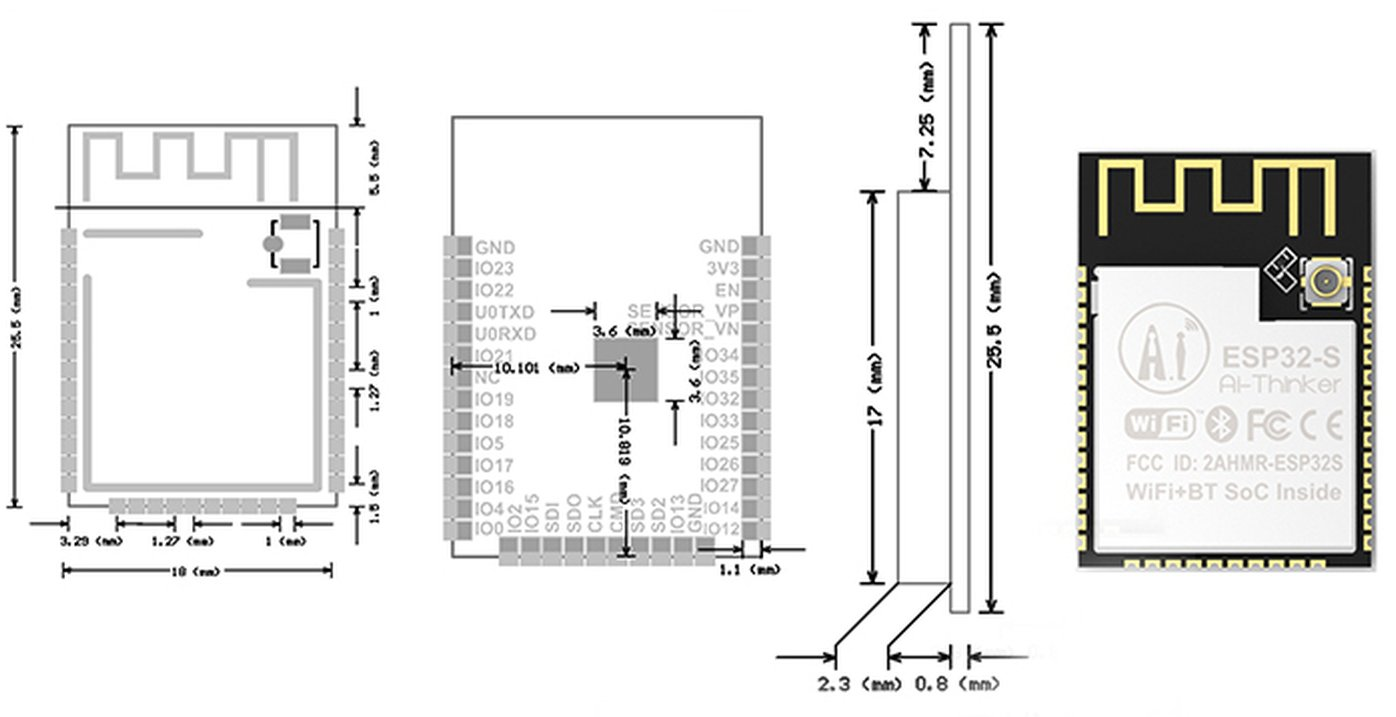
\includegraphics[width=0.7\textwidth]{img/esp32.jpg}
              \caption{Schemat wykorzystanej jednostki centralnej}
              \label{esp}
            \end{figure}
    
            Warto zwrócić uwagę na fakt, że wybrana jednostka obliczeniowa posiada dość imponujące parametry jak na tak tani produkt. Pozwoli to na zadowalającą wydajność
            całego systemu bez obaw o niewystarczające zasoby lub kiepską optymalizację.
    
    
        \section{System operacyjny}
            Jednym z wielu wyzwań stawianych przed programistą systemów wbudowanych jest stworzenie rozbudowanego programu wykonującego wiele zadań na pojedynczej jednostce obliczeniowej. Powoduje to konieczność wykorzystywania rozbudowanych maszyn stanów i bardzo skomplikowanej logiki. Z pomocą przychodzą systemy operacyjne, które umożliwiają tworzenie programów wielowątkowych i uprzyjemniają korzystanie z procesorów rdzeniowych. Ze względu na to że użyty w projekcie procesor ma dwa rdzenie logiczne oraz że program ten powinien wykonywać wiele czynności jednocześnie, błędem byłoby nie skorzystać dobrodziejstw oferowanych przez systemu operacyjne. Program wykonuje się więc pod kontrolą otwarto źródłowego systemu czasu rzeczywistego FreeRTOS \cite{freertos}. Jest on znany z dużej szybkości działania. Implementuje on wszystkie elementy niezbędne do pracy z wieloma procesami takie jak muteksy, semafory czy kolejki priorytetowe. Bez niego obsługa WiFi czy protokołu MQTT byłaby niewyobrażalnie skomplikowana i czasochłonna. 
            
            Mówiąc o zaletach systemów operacyjnych warto też wspomnieć o ich wadach. Najważniejszą z nich jest narzut obliczeniowy wynikający między innymi z pracy planisty. Z tego powodu część czasu procesora poświęcana jest na pracę samego systemu i nie bierze udziału w wykonywaniu obliczeń na rzecz programu. Jest to jednak niska cena za tak potężne narzędzie znacznie ułatwiające tworzenie programu.
      
            
        \section{Framework}
            Przy opracowywaniu kodu źródłowego sterownika został użyty framework ESP-IDF \cite{esp-idf} przygotowany przez producenta procesora. Na stronie dostawcy tego rozwiązania można znaleźć także obszerną dokumentację tłumaczącą wykorzystanie frameworka w praktyce wraz z wieloma przykładami użycia. Zastosowanie gotowej abstrakcji zdejmuje z dewelopera obowiązek implementacji wielu skomplikowanych aspektów programu. W tym projekcie szczególnie przydatna jest implementacja stosu TCP/IP i protokołu MQTT.
    
    
        \section{Schemat funkcjonowania}
            % TODO  diagram wątków, kolejki
            Największą zaletą posiadania systemu operacyjnego jest możliwość tworzenia osobnego procesu dla każdego zadania. To znowu pozwala dokładnie kontrolować czasy wywołań i częstotliwości odpowiednich wydarzeń. Główne zadania stawiane temu sterownikowi to:
            
            \begin{itemize}
                \item obsługa silnika wraz z liczeniem PID,
                \item pomiary napięcia zasilania,
                \item wysyłanie danych przez MQTT,
                \item obsługa WiFi, odbieranie danych z MQTT, planista i obsługa przerwań
            \end{itemize}
            
            W ten sposób kształtują się cztery główne procesy, które biorą udział w pracy systemu:
            
            \begin{description}
                \item [Pierwszy] Proces ten wykonuje się dokładnie co 10ms. Każde odchylenie w czasie tego procesu powodowałoby niedokładną pracę regulatora PID, co skutkowałoby niestabilnym zachowaniem się silnika. Z tego też powodu, ten proces został na stałe przypięty do pierwszego rdzenia procesora oraz otrzymał bardzo wysoki priorytet. Jego schemat działania został zamieszczony na rys. \ref{fig:pid_plantuml} 
                
                \item [Drugi] Ten proces odpowiedzialny jest za pomiary zasilania. Wykonuje się co około 20ms, ale ze względu na ustawiony bardzo niski priorytet ustępuje każdemu innemu zadaniu. Wykonuje się więc tylko gdy procesor nic innego nie robi. Nie stanowi to żadnego problemu, ponieważ opóźnienia w wykonywaniu tego procesu nie wpływają z znacznym stopniu na prawidłową pracę systemu. Informacja przez niego generowana trafia wyłącznie na panel kontrolny użytkownika i jest wyświetlana w aplikacji dostępowej, gdzie aktualizowana jest z częstotliwością około 5Hz. Drobne odchyły w czasie aktualizacji są więc niewykrywalne. Proces ten został przypięty do rdzenia numer 2.
                
                \item [Trzeci] Zadaniem tego procesu jest odbieranie danych z kolejek priorytetowych FIFO i wysyłanie ich poprzez protokół MQTT do brokera. Otrzymał on średni priorytet. Wykonuje się w momencie gdy, w którejś z kolejek pojawiają się jakieś nowe dane. On również został przypisany do rdzenia numer 2. Jako jedyny z tych procesów zaczyna swoją pracę dopiero po nawiązaniu poprawnego połączenia z serwerem MQTT. Wraz z zerwaniem połączenia jest on usuwany.
                
                \item [Czwarty] Ostatni proces jest głównym procesem w systemie. Odpowiada on za początkową konfigurację peryferiów przy starcie systemu. Z niego wywodzi się także reszta procesów. Po poprawnym starcie oraz inicjalizacji peryferiów zostaje on zawieszony.
            \end{description}
            
            W systemie istnieją także inne procesy zajmujące się między innymi obsługą połączenia z siecią, klientem MQTT, przerwaniami oraz planistą systemu. 
            

        \section{Mostek H}
        % TO DO
            Głównym zadaniem mikrokontrolerów jest zbieranie danych z czujników, wykonywanie obliczeń i podejmowanie decyzji. Nie zostały jednak stworzone do sterowania elementami o wyższym napięciu czy dużych prądach. Wyjścia mikrokontrolerów potrafią dostarczyć zazwyczaj około kilkudziesięciu miliamperów prądu. W przypadku mikrokontrolera użytego w projekcie dokumentacja \cite{esp32} informuje o bardzo wysokim prądzie wyjściowym dochodzącym nawet do 40mA w sprzyjających warunkach. Jest to wystarczająca ilość do zasilenia diody LED (ok. 20mA) czy sterowania tranzystorem. Z drugiej strony jest to wielokrotnie za mało, aby sterować silnikiem prądu stałego. Takie silniki zazwyczaj nie dość że działają na wyższych napięciach aniżeli 3.3V to często potrafią zużyć ponad 2A prądu podczas obciążenia. Jednym ze sposobów kontrolowania prędkości obrotowej takiego jest zastosowanie wcześniej wspomnianego tranzystora lub przekaźnika. Minusem takiego rozwiązania jest brak możliwości zmiany kierunku obrotów. Rozwiązaniem, które pozwoli na sterowanie silnikiem w obu kierunkach najczęściej jest użycie mostka H. Jego schemat przedstawiono na rys. \ref{fig:h_bridge_schematic}
            
            \begin{figure}[ht]
                \centering
                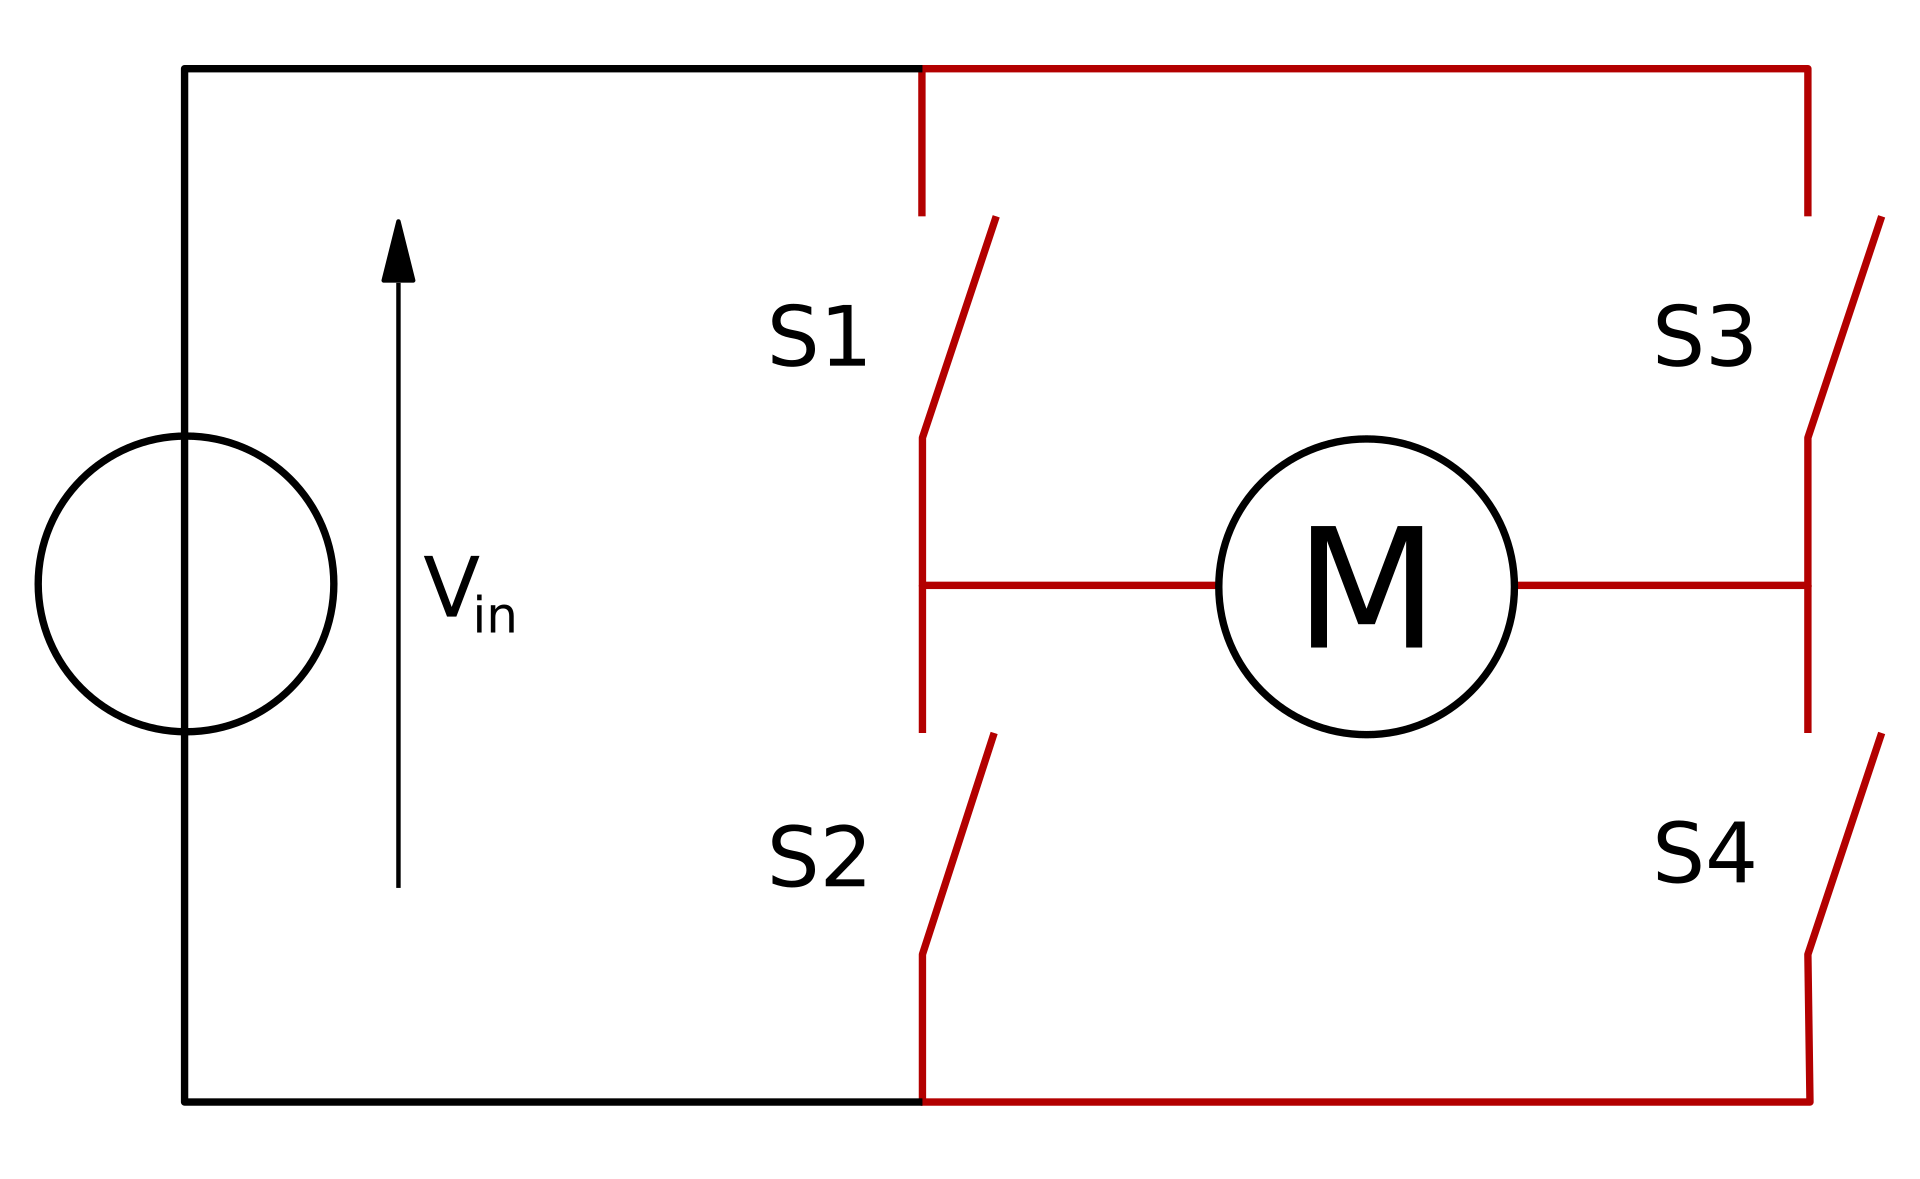
\includegraphics[width=0.7\textwidth]{img/h_bridge_schametic.png}
                \caption{Ogólny schemat mostka H}
                \label{fig:h_bridge_schematic}
            \end{figure}
            
            W roli mostka H został wyselekcjonowany bardzo popularny układ scalony L298N w obudowie Multiwatt15. Nie jest to nowy układ scalony, ale jest on przetestowany i zdecydowanie wystarczający dla tego zastosowania. Może się on poszczycić napięciem zasilania silników do 46V i prądem szczytowym na poziomie 2A. W rzeczywistości posiada on dwa osobne kanały co sprawia że z jego pomocą możliwe jest jednoczesne sterowanie dwoma silnikami, jednakże projekt ten zakłada wykorzystanie tylko jednego silnika, więc drugi kanał pozostanie nieaktywny. Może to spowodować wolniejsze nagrzewanie się układu, co z pewnością przełoży się na jego stabilniejszą pracę. 
            
            Układ scalony tego typu został przedstawiony na rys. \ref{fig:h_bridge}. Redukuje on znacząco poziom skomplikowania urządzenia ponieważ w celu uruchomienia go wystarczą cztery diody redukujące prądy indukowane na cewkach silników podczas ich pracy oraz kondensator filtrujący zasilanie \cite{mostek}. Przykładowe podłączenie jest zaprezentowane na rys. \ref{fig:h_bridge_connection}.
            
            \begin{figure}[ht]
                \centering
                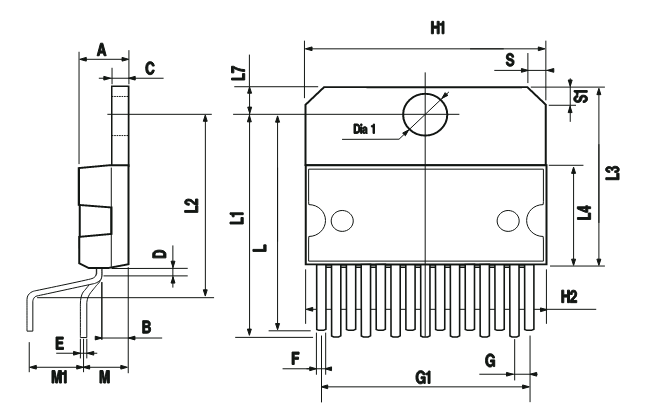
\includegraphics[width=0.7\textwidth]{img/h_bridge.png}
                \caption{Schemat wykorzystanego mostka H}
                \label{fig:h_bridge}
            \end{figure}
            
            \begin{figure}[ht]
                \centering
                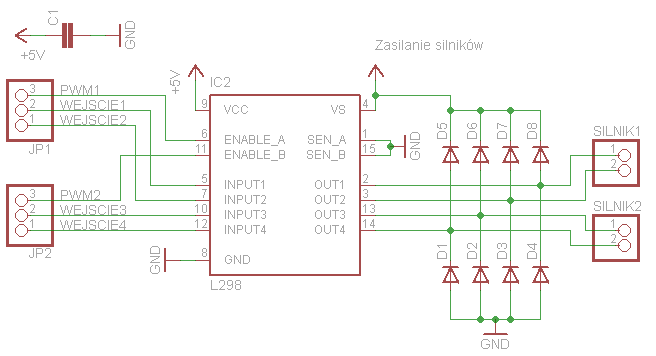
\includegraphics[width=0.7\textwidth]{img/h_bridge_connection.png}
                \caption{Schemat podłączenia mostka H}
                \label{fig:h_bridge_connection}
            \end{figure}
            
        \section{Silnik}
            Silnik jest to bardzo konkurencyjnie wyceniany produkt firmy DFROBOT. Został on wybrany w głównej mierze ze względu na swoją niską cenę i parametry, które w zupełności wystarczą do zrealizowania tego projektu. Jest on wyposażony w metalową przekładnię zapewniającą przełożenie napędu w proporcji 20:1. Ponadto, na końcu silnika znajduje się fabrycznie zamontowany enkoder kwadraturowy, który produkuje 11 impulsów na każdy obrót wałka głównego. Schemat silnika wraz z enkoderem umieszczony został na rys. \ref{fig:engine}
            
            \begin{figure}[ht]
                \centering
                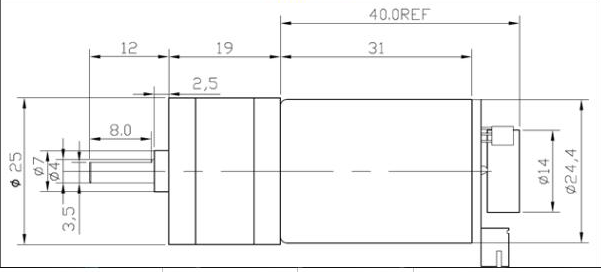
\includegraphics[width=0.9\textwidth]{img/silnik.png}
                \caption{Schemat wykorzystanego silnika}
                \label{fig:engine}
            \end{figure}


        \section{Płytka drukowana}
            \subsection{Opis}
                Urządzenie wykonawcze zawiera mikrokontroler, mostek H oraz element wykonawczy w postaci silnika prądu stałego wyposażonego w enkoder kwadraturowy. Poza możliwością zadawania napięcia na silnik, urządzenie dysponuje funkcją pomiaru napięcia zasilania. Poza wymienionymi jednostkami na płytce drukowanej znajdują się także wszystkie elementy niezbędne do prawidłowej pracy procesora takie jak kondensatory i rezystory. Obie strony płytki zarówno górną jak i dolną  zostały dołączone do projektu.
          
            \subsection{Wygląd}
                Przygotowany wzór płytki drukowanej z rozlokowanymi elementami i poprowadzonymi ścieżkami został złączony do tego dokumentu. Obie strony płytki zarówno górna jak i dolna dostępne są jako rysunek \ref{fig:pcb}.
                
                \begin{figure}[ht]
                    \centering
                    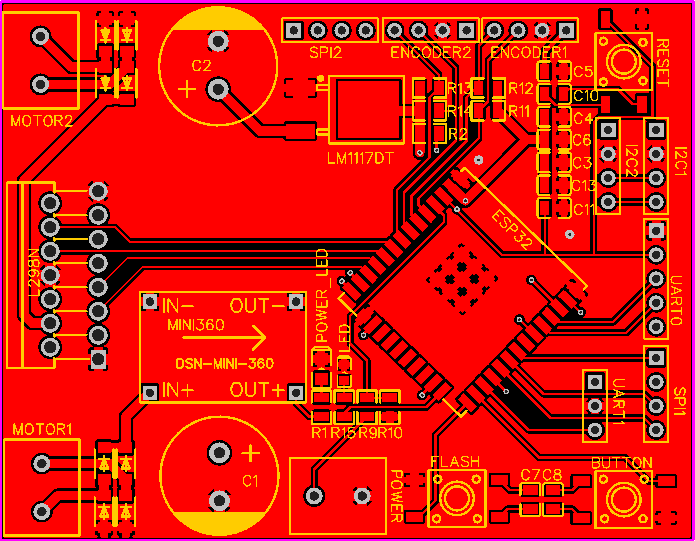
\includegraphics[width=0.8\textwidth]{img/pcb_front.png}
                    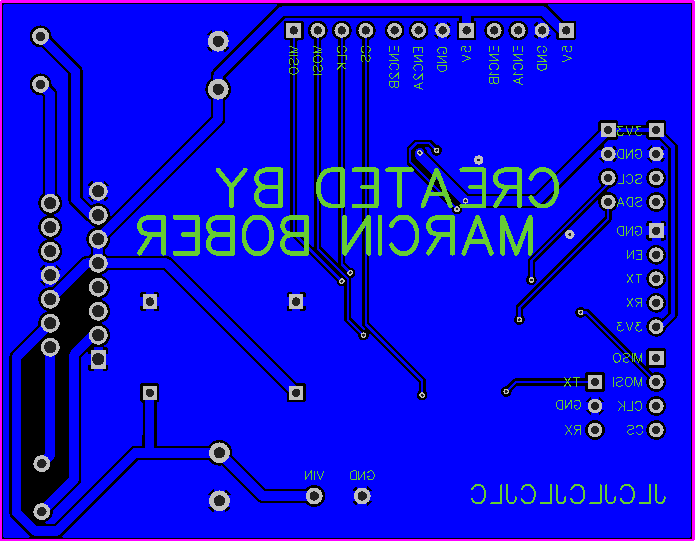
\includegraphics[width=0.8\textwidth]{img/pcb_back.png}
                    \caption{Wygląd PCB}
                    \label{fig:pcb}
                \end{figure}
    
            \subsection{Schemat}
                Schemat składa się z trzech stron. Pierwsza strona (rys. \ref{fig:pcb_schematic_1}) dotyczy sekcji zasilania oraz połączeń z SoC wraz z elementami niezbędnymi do jego prawidłowej pracy. Druga strona (rys. \ref{fig:pcb_schematic_2}) opisuje połączenia enkoderów oraz mostka H. Trzecia strona (rys. \ref{fig:pcb_schematic_3}) są to jednie wyprowadzenia interfejsów.
                  
                \begin{landscape}
                    \begin{figure}
                      \centering
                      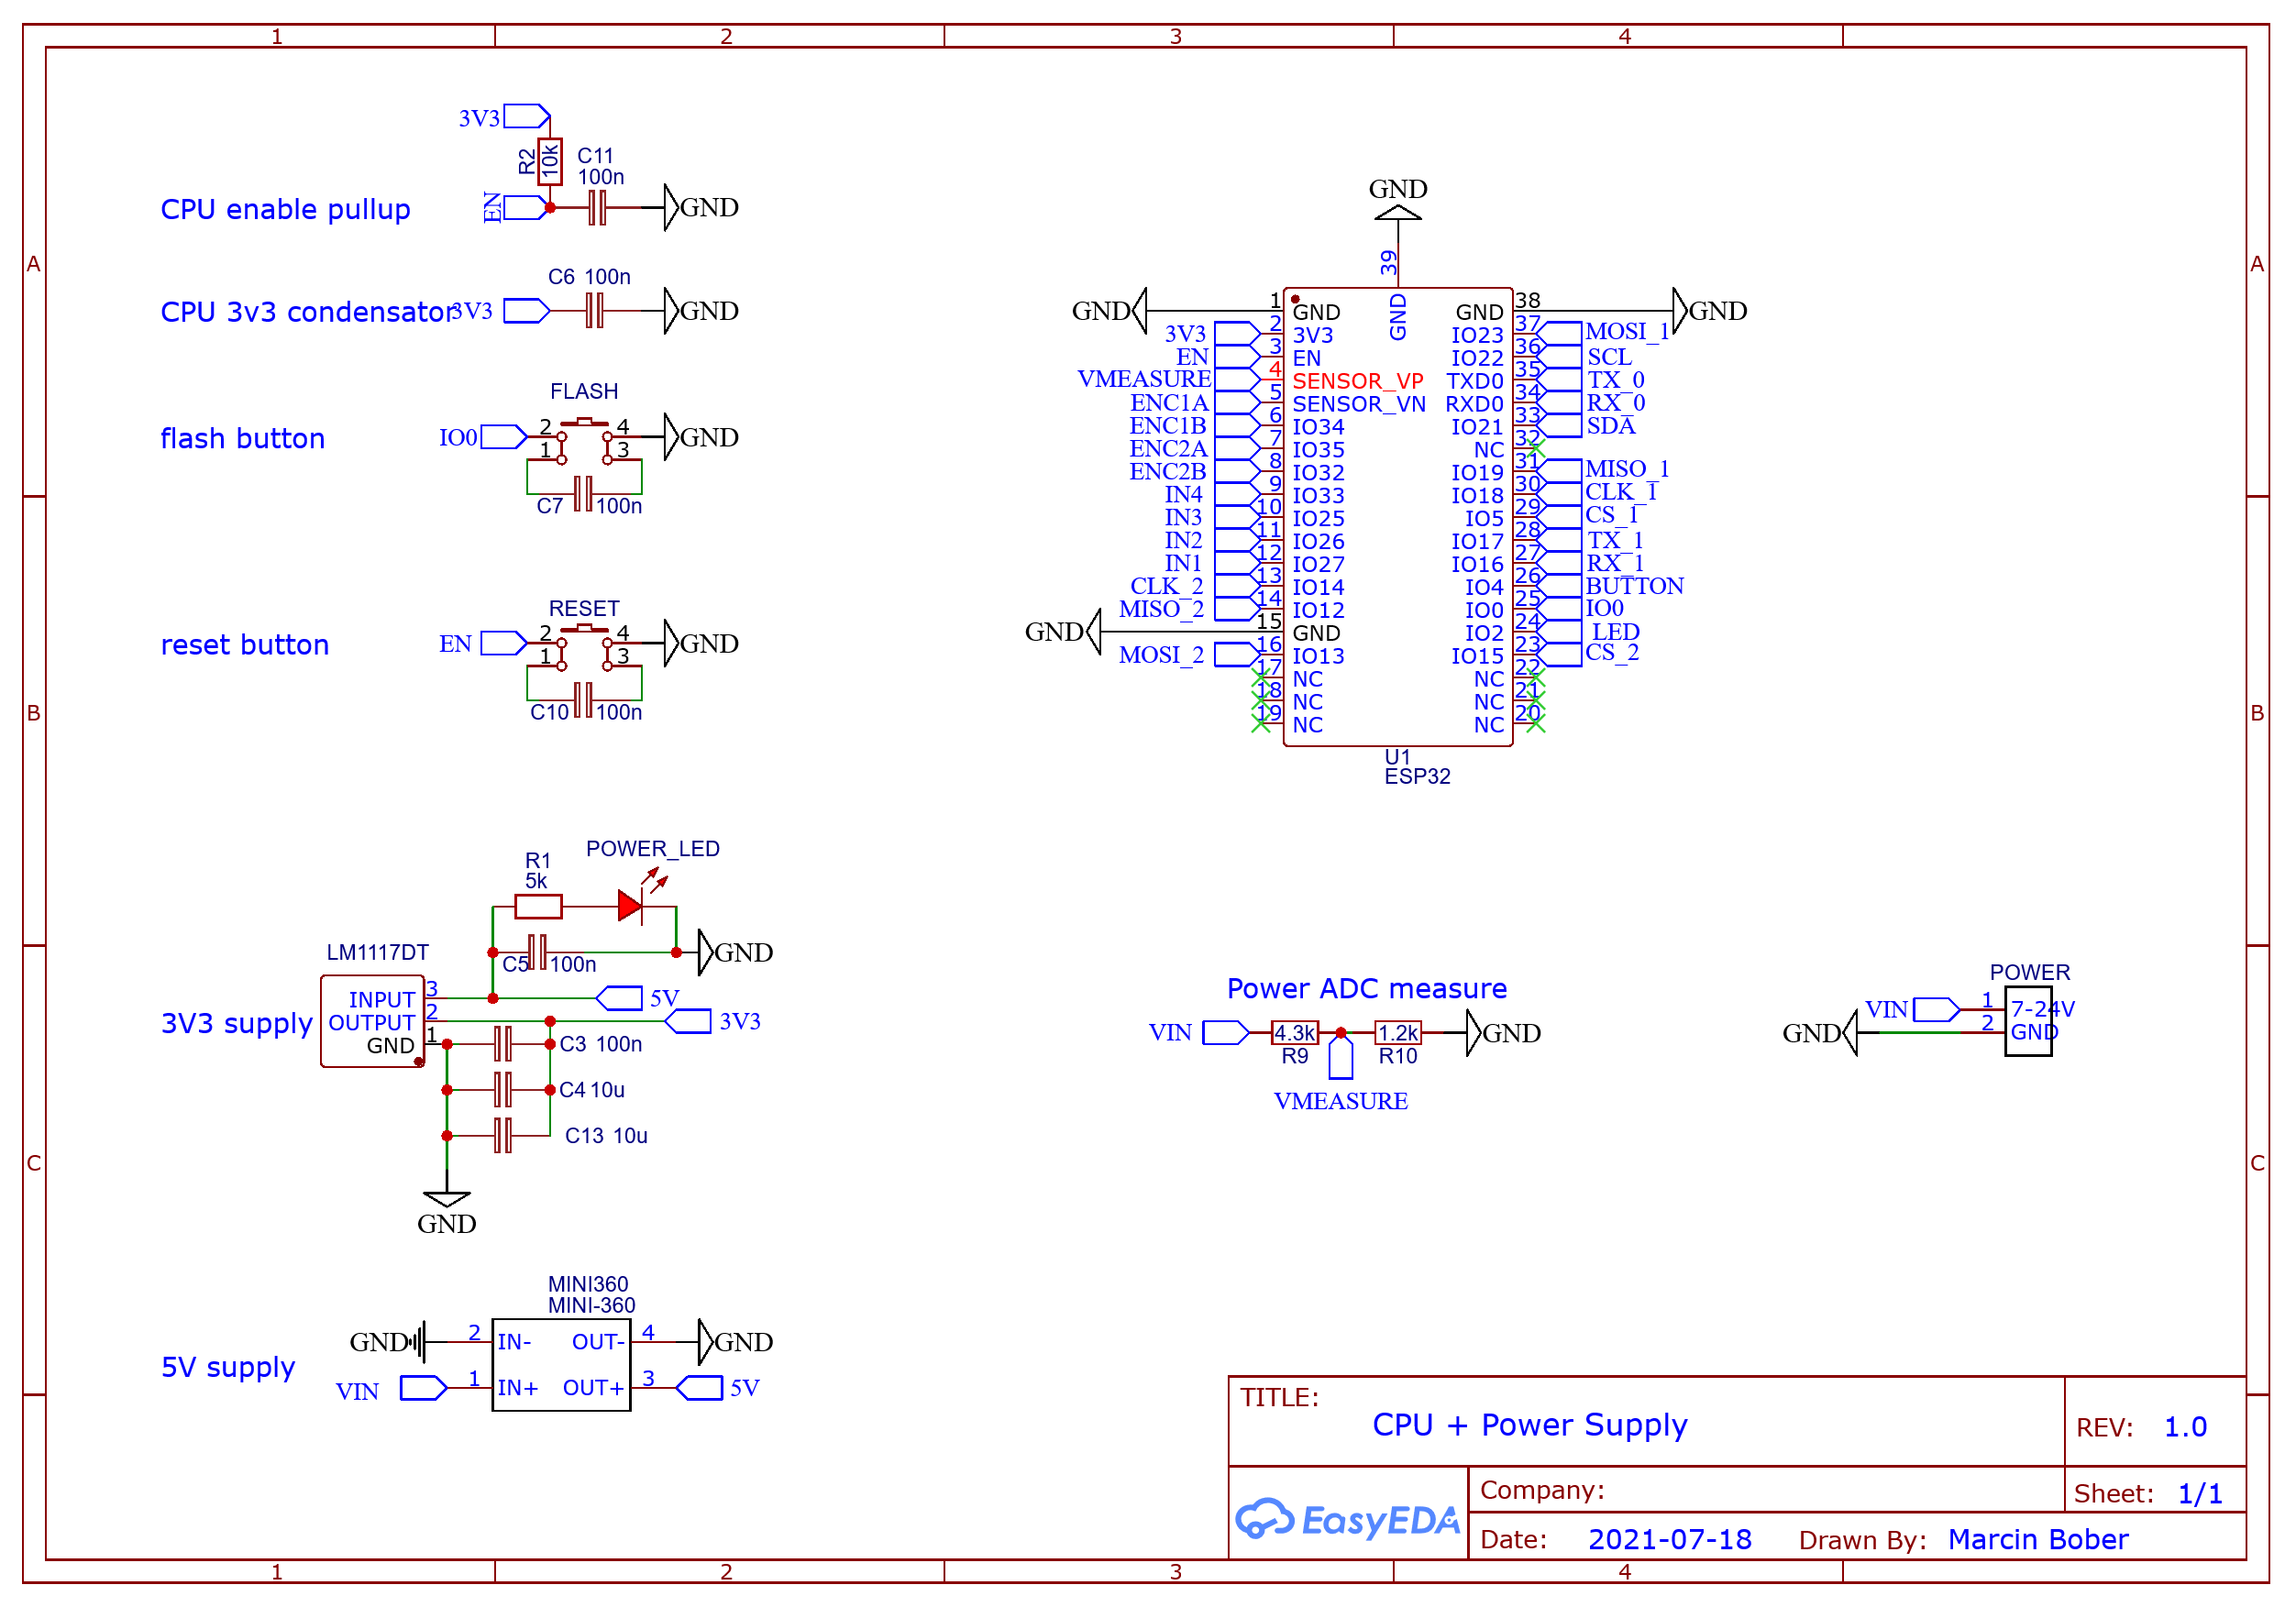
\includegraphics[width=0.85\textwidth]{img/pcb1.png}
                      \caption{Schemat płytki PCB (CPU+PSU)}
                      \label{fig:pcb_schematic_1}
                    \end{figure}
                \end{landscape}
                
                \begin{landscape}
                    \begin{figure}
                      \centering
                      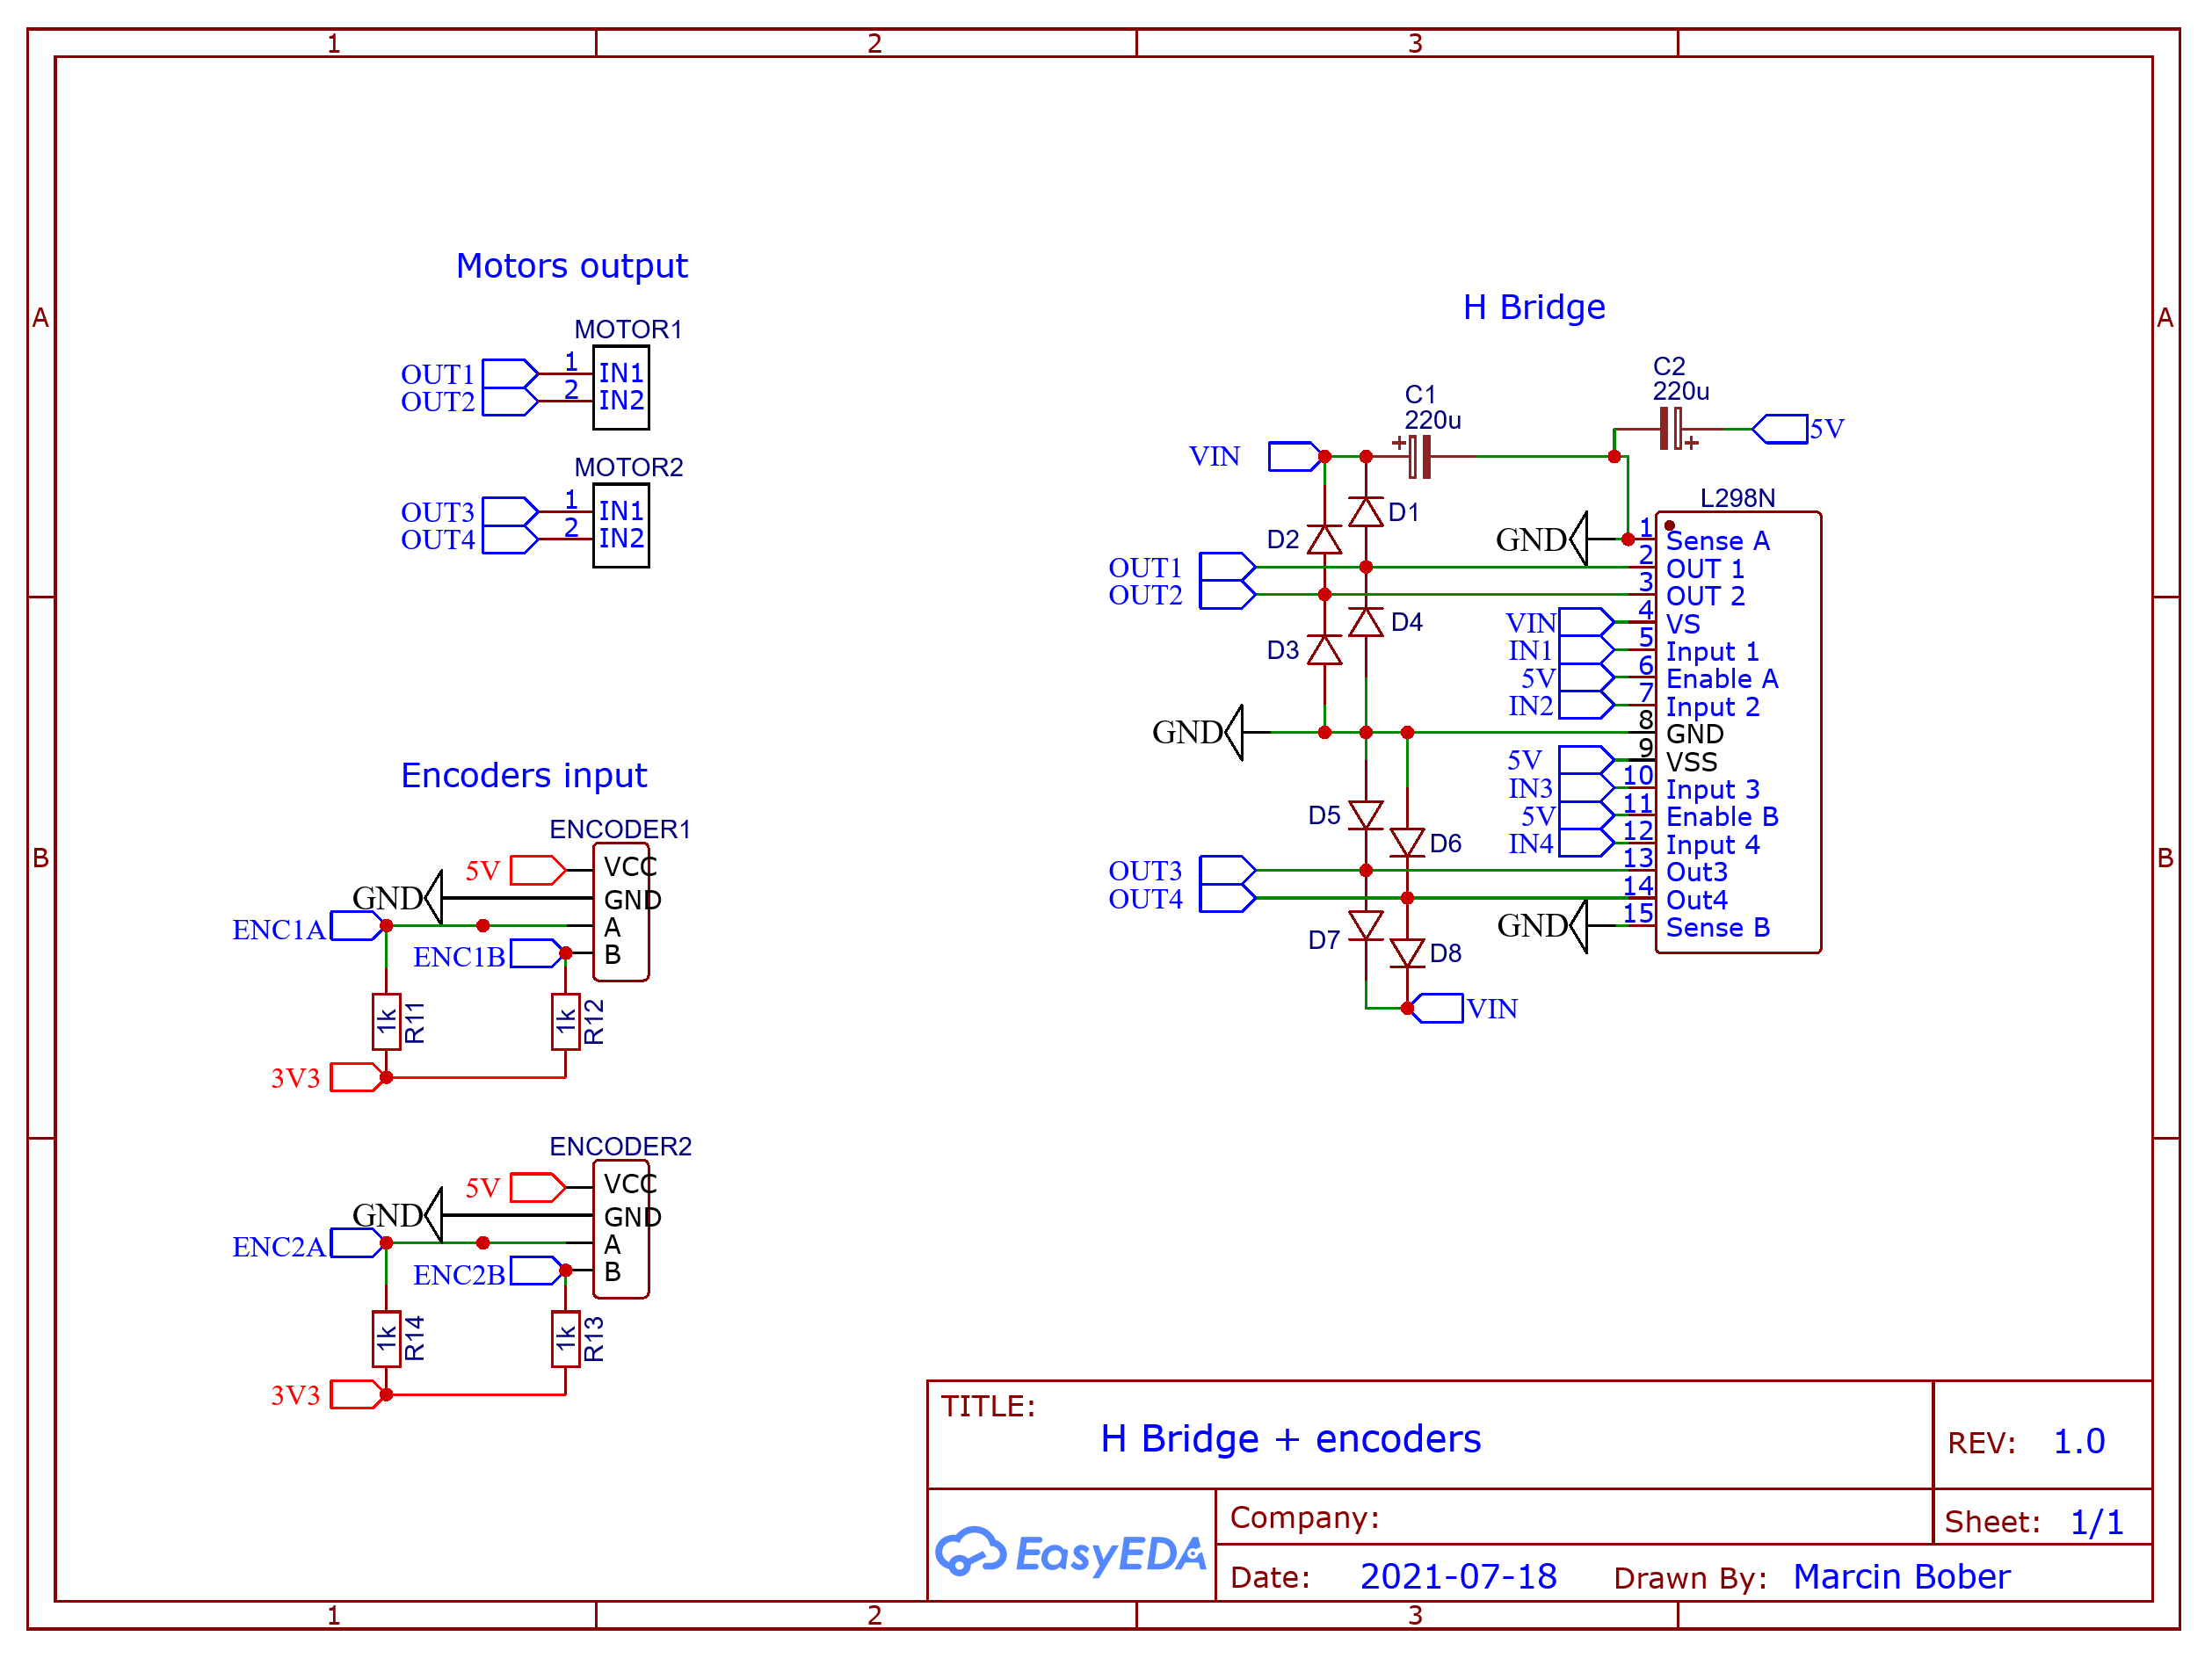
\includegraphics[width=0.80\textwidth]{img/pcb2.png}
                      \caption{Schemat płytki PCB (mostek + enkodery)}
                      \label{fig:pcb_schematic_2}
                    \end{figure}
                \end{landscape}
        
                \begin{landscape}
                    \begin{figure}
                      \centering
                      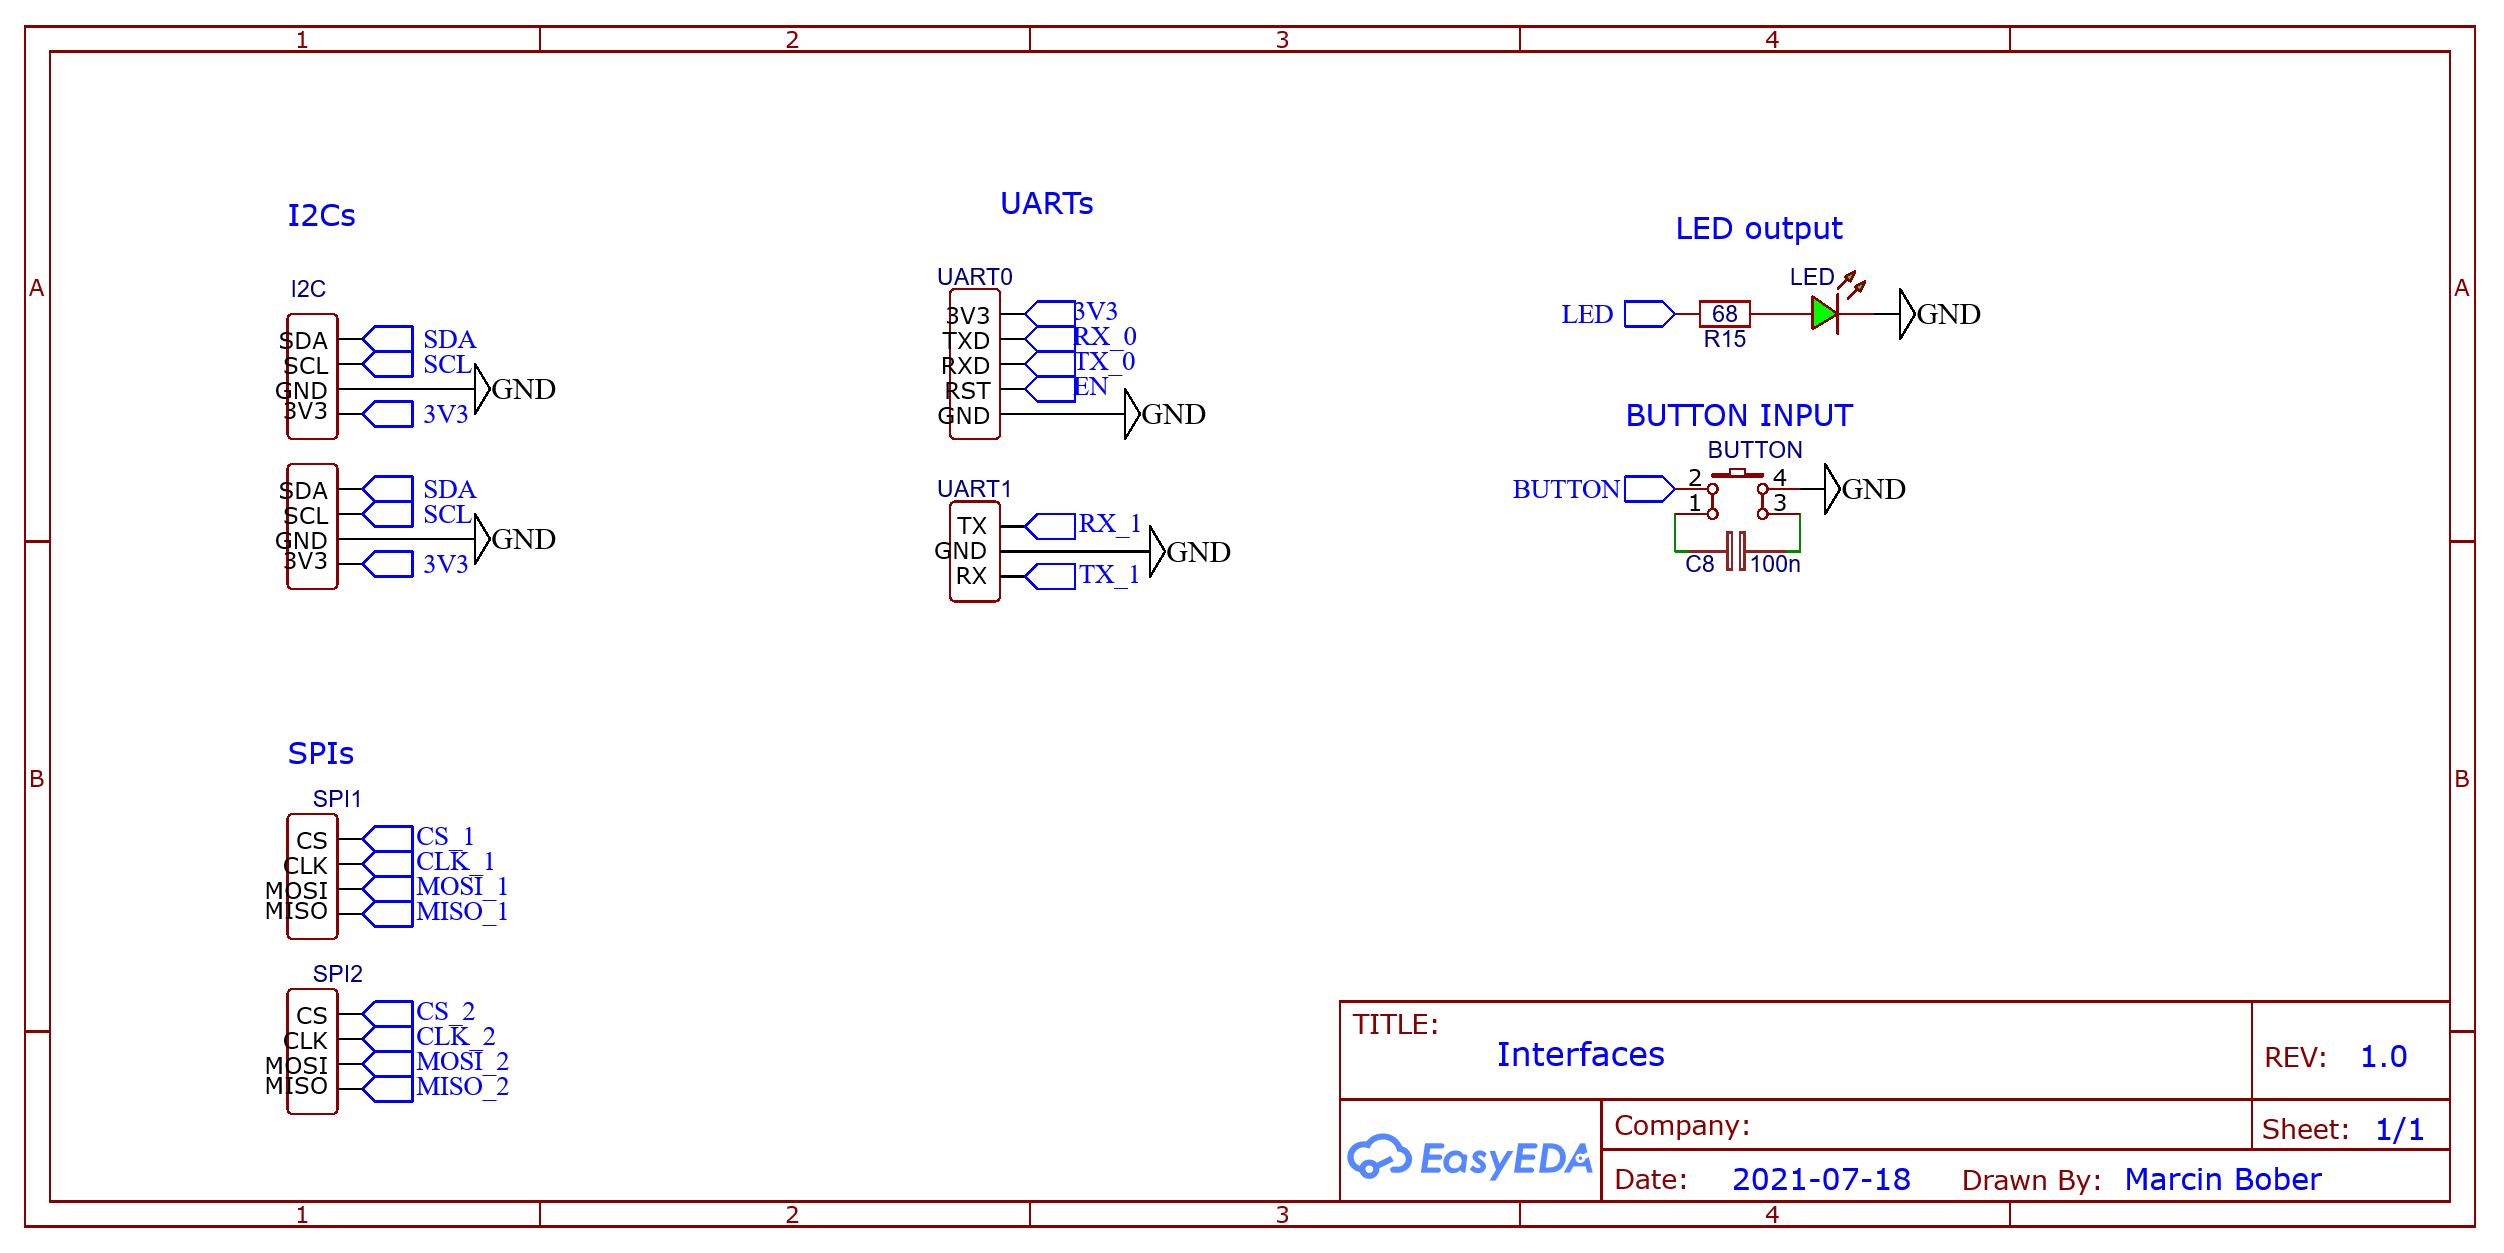
\includegraphics[width=0.85\textwidth]{img/pcb3.png}
                      \caption{Schemat płytki PCB (interfejsy)}
                      \label{fig:pcb_schematic_3}
                    \end{figure}
                \end{landscape}
        
    
    
